% -- Document configuration
\documentclass{article}

% -- Input and language settings
% \usepackage[utf8]{inputenc}
\usepackage[spanish]{babel}
\decimalpoint                             % From babel package to use points instead of commas in decimals

% -- Page and line settings
\usepackage{geometry}
\geometry{letterpaper, 
    % margin=2cm, 
    left=3cm, right=3cm,
    top=1.2cm, bottom=1.2cm,
    includefoot, 
    includehead}
\renewcommand{\baselinestretch}{1.2}

% -- Required packages
\usepackage{xcolor}
\usepackage[many]{tcolorbox}
\usepackage{mathtools,amsfonts,amsmath}     % Loads amsmath if not already loaded
\allowdisplaybreaks                         % To allow page breaks if equations are too long
\usepackage[parfill]{parskip}               % No indent and separation lines for paragraphs
\usepackage{cancel}                         % To cancel math terms
\usepackage[shortlabels]{enumitem}          % To handle enumerations
\usepackage{tikz}
\usetikzlibrary{automata, arrows.meta, positioning}
\usepackage[mode=buildnew]{standalone}      % To import figures in standalone files
\usepackage[hidelinks]{hyperref}
\usepackage[spanish]{cleveref}              % To use autocompleted reference labels, language must be change as in babel package
\usepackage{caption}                        % Caption and subcaption to allow subfigures
\usepackage{subcaption}
\usepackage{float}                          % To specify the location of figures
\usepackage{multicol}                       % To use multicolumns
\usepackage[bottom]{footmisc}               % To locate footnotes at the bottom

% -- Title and heading settings
\usepackage{titling}
\usepackage{fancyhdr}
\pagestyle{fancy}

% -- Code and code formatting
\usepackage{minted}                         % To insert code
\usemintedstyle[julia]{gruvbox-light}       % Code theme and language
\definecolor{bg}{rgb}{0.98, 0.97, 0.88}     % Code block background

\usepackage{fontspec}                       % To allow the use of monospace fonts
\setmonofont{JuliaMono}[Path=./codefonts/, Extension=.ttf, UprightFont=*-Regular, ItalicFont=*-RegularItalic, Scale=0.75]

\usepackage{fancyvrb}                       % To change line number font
\renewcommand{\theFancyVerbLine}{\textcolor{gray}{\footnotesize\texttt{\arabic{FancyVerbLine}}}}

\definecolor{light-gray}{gray}{0.95}        % Color, box and style to show small code thingys inside normal text
\newcommand{\code}[1]{\colorbox{light-gray}{\texttt{#1}}}

% -- Bilbiography preferences
\usepackage[square,numbers]{natbib}
\bibliographystyle{unsrt}

% -- Footnotes without numbering
\newcommand\nnfootnote[1]{%
  \begin{NoHyper}
  \renewcommand\thefootnote{}\footnote{#1}%
  \addtocounter{footnote}{-1}%
  \end{NoHyper}
}

% -- Theorems
\newtheorem{theorem}{Theorem}

\lhead{\theinstitution\ -- \thedepartment}
\chead{}
\rhead{Programación para la IA\ -- \thetitle}
\lfoot{}
\cfoot{\thepage}
\rfoot{}

% -- Problem solution
\newenvironment{solution}
{\begin{quote}
\textbf{Solución:}\medskip

}
{

\hfill\rule{0.5\textwidth}{0.5pt}
\end{quote}}

% -- Equation result
\newcommand{\result}[1]
{
\tcbhighmath[colframe=white, colback=gray!15, sharp corners]
{#1}
}

% -- Function definitions
\newcommand{\dprod}[2]{{#1} \cdot {#2}}
\newcommand{\txtgray}[1]{\textcolor{gray}{#1}}

% -- Author information
\title{Actividad 5}
\author{Leonardo Flores Torres}
\newcommand\theinstitution{Universidad Veracruzana}
\newcommand\thedepartment{Inteligencia Artificial}
\newcommand\thecourse{Programación para la Inteligencia Artificial}

% -- Paths
% \newcommand\codelists{../programs/lists.rkt}

% Remove red color boxes of "syntax errors" in minted
\AtBeginEnvironment{minted}{%
  \renewcommand{\fcolorbox}[4][]{#4}}

\newcommand{\diannao}{\texttt{diannao}}
\newcommand{\hongdiannao}{\texttt{hongdiannao}}

% -- Document
\begin{document}

\thispagestyle{empty}

%Title
\begin{center}
\textsc{\theinstitution}\\[2mm]

\thedepartment

\rule{0.6\textwidth}{0.5pt}\\[2mm]

\thecourse \\[4mm]

{\Large \textbf{\thetitle}}\\[2mm]

\theauthor \\[2mm]

{\small \today}
\end{center}
\medskip

% -- 
\vspace{1cm}

\textbf{%
Programar un algoritmo de su elección (no tan sencillo) y analizarlo de la siguiente forma:}
\begin{enumerate}
    \item Graficar el tiempo de ejecución en función de $N$,
    \item sobre los mismos ejes graficar 2 cotas superiores y dos cotas inferiores,
    \item repetir el punto 1 y 2 ejecutando el programa en otra computadora de distinto desempeño,
    \item analizar los resultados y discutirlos. Escribir de la manera más completa las características de las 2 computadoras.
\end{enumerate}

\vspace{1cm}

El algoritmo que se eligió fue computar un fractal, más específicamente, el fractal que se genera a partir del set de Mandelbrot. Las propiedades del fractal de Mandelbrot han sido estudiadas considerablemente, tan es así que en este trabajo se usa para estudiar los efectos computacionales de implementar un algoritmo para generarlo.

\begin{figure}[ht!]
    \centering
    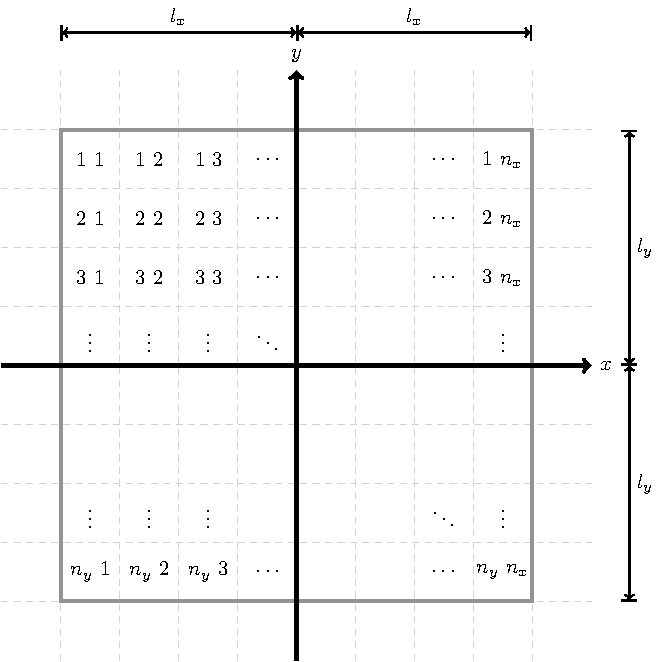
\includegraphics[scale=0.8]{../figures/grid/grid}
    \caption{Discretización del espacio}
    \label{fig:grid}
\end{figure}

El set de Mandelbrot se conoce como el conjunto de puntos generado a partir de 
\begin{equation*}
    z_{n+1} = z_{n}^2 + c
\end{equation*}
donde ambos $z$ y $c \in \mathbb{C}$. Pero no todos los puntos $z_i$ pertenecen al conjunto, solamente aquellos que $|z_i| \leq 2$, esto quiere decir que no es necesario computar todos los valores dentro de un dominio de cardinalidad infinita como lo es $\mathbb{C}$. Una manera útil de interpretar esta restricción es que solamente los números $z_i$ que estén dentro de un círculo centrado en el origen de radio 2 pueden pertenecer al conjunto.

Quisisera tomarme la libertad acerca de cómo fue que construí el algoritmo. Encontré varias fuentes en internet tales como un post en el sitio \href{https://www.codingame.com/playgrounds/2358/how-to-plot-the-mandelbrot-set/mandelbrot-set}{CodinGame}, y en el sitio popular de tutoriales de \code{python}, \href{https://realpython.com/mandelbrot-set-python/#making-an-artistic-representation-of-the-mandelbrot-set}{RealPython}. A pesar de incluir sus códigos faltaba la explicación que considero yo más importante, aquella que trata la discretización del espacio más allá de solamente definir una matriz de pixeles con ciertas dimensiones.

Primero se debe comenzar con una representación del espacio como se muestra en la \cref{fig:grid} donde el grid tiene una anchura de $2 l_x$, y una altura de $2 l_y$. En los lenguajes de programación es común que al tratar con una imágen sus pixeles estén ordenados como se muestra en la imagen anteriormente mencionada. Esto asemeja a una matriz, sí, una matriz de pixeles donde cada entrada de la matriz tiene dos elementos importantes a considerar. Los índices de las entradas en la matriz, y el valor del color que cada entrada contiene, ya sea en RGB, HSV, u otro.

\begin{figure}[ht!]
    \centering
    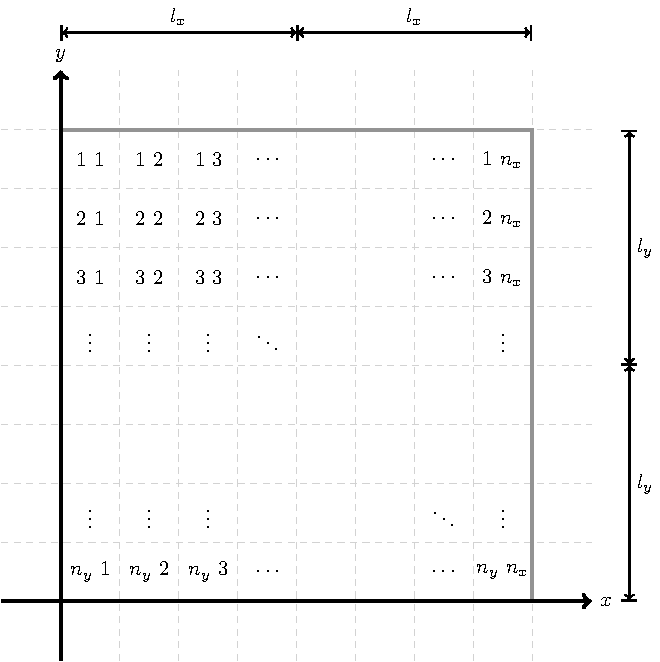
\includegraphics[scale=0.75]{../figures/grid-translated/grid-translated}
    \caption{Traslación aplicada al espacio discretizado.}
    \label{fig:grid-moved}
\end{figure}

En este punto todavía es algo confuso sobre cómo trabajar con los índices de la matriz para generar las coordenadas necesarias para realizar el cómputo de $z_i$. Es importante clarificar que el eje-$y$ es el eje de la componente imaginaria de $z_i$, $Im(z_i)$, mientras que en el eje-$x$ se encuentran las componentes reales $Re(z_i)$ ¿Que tal si se hace una traslación de las coordenadas para que un vértice de nuestro espacio discretizado coincida con el origen de coordenadas? La traslación elegida fue $x' = x - l_x$, y $y' = y - l_y$. Nótese que por la restricción inicial $|z_i| \leq 2$ se deriva que $l_x \leq 2$ y $l_y \leq 2$.

Después de la traslación, \cref{fig:grid-moved}, pareciera ser mas intuitivo cómo debe uno moverse en el espacio para moverse entre vértices de pixeles. Por ejemplo, si quisiera moverme al pixel en la primera fila y tercera columna hay dos opciones. Si comenzara a moverme en el vértice superior izquierdo de mi espacio podría moverme una distancia $3 \Delta x$ y ninguna en $y$ lo que me posicionaría tocando al pixel $[1,\ 3]$ en su vértice superior derecho, o podría moverme $2 \Delta x$ y $\Delta y$ para encontrarme en el vértice inferior izquierdo del mismo pixel. Nuestra intuición va bien encaminada, solamente necesita de un paso más.
\begin{figure}[ht!]
    \centering
    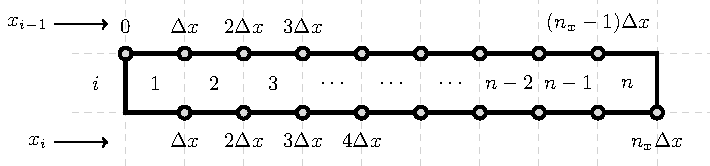
\includegraphics[scale=0.75]{../figures/small-grid/small-grid}
    \caption{Movimiento entre los vértices de pixeles en una fila cualquiera dentro de la imagen.}
    \label{fig:small-grid}
\end{figure}

No se ha mencionado porque ha sido ilustrado en las \cref{fig:grid,fig:grid-moved} pero los pixeles representan un movimiento desde un vértice a otro vértice de tamaños $\Delta x$ o $\Delta y$ dependiendo si nos movemos a lo largo del eje-$x$ ó del eje-$y$, donde
\begin{equation*}
    \begin{split}
        \Delta x & = \frac{2 l_x}{n_x}\ , \\
        \Delta y & = \frac{2 l_y}{n_y}\ ,
    \end{split}
\end{equation*}
y $n_x$, $n_y$, representan el número de divisiones del espacio lo cual es equivalente al número de pixeles en el que se divide la imagen a lo largo de los ejes.

Retomando el ejemplo anterior, las dos maneras de comenzar el movimiento entre vértices se ilustra en la \cref{fig:small-grid} para una fila cualquiera de pixeles dentro de la imagen, lo mismo aplica para el movimiento entre pixeles en una columna cualquiera. Ahora, los índices que se tenían en un inicio nos dicen algo, dependiendo del índice será la posicion en la que estaremos con movimientos de longitud $\Delta x$,
\begin{equation*}
    \begin{split}
        x_{i-1} & = (i - 1) \Delta x\ , \\
        x_{i} & = i \Delta x\ ,
    \end{split}
\end{equation*}
donde $i=1, 2, 3, \ldots, N$. Además, $N$ puede ser $n_x$ ó $n_y$ dependiendo de la dirección del movimiento. Lo mismo es cierto en la dirreción del eje-$y$. Ahora, si tomamos $x_i$ y $x_{i-1}$ podemos encontrar el punto medio, aquel que se encuentra justo en el centro del pixel
\begin{equation*}
    \begin{split}
        x_{c}^{i} & = \frac{x_i + x_{i-1}}{2} = \frac{i \Delta x (i-1) \Delta x}{2}\ , \\
        & = \Delta x \frac{(2i - 1)}{2} = \frac{2 l_x}{2} \frac{(2i - 1)}{2}\ ,\\
        x_{c}^{i} & = \frac{l_x}{n_x} (2i - 1)\ .
    \end{split}
\end{equation*}
De igual manera,
\begin{equation*}
    y_{c}^{i} = \frac{l_y}{n_y} (2i - 1)\ .
\end{equation*}
De aquí que podemos acceder a cualquier elemento dentro de nuestra matriz de pixeles partiendo de sus índices para obtener sus coordenadas $(x_{c}^{i}, y_{c}^{i})$ ¿Recuerda usted la traslación hecha anteriormente? Tenemos que regresar a nuestro sistema de coordenadas iniciales, esto se obtiene al movernos de regreso una distancia $l_x$ en el eje-$x$, y una distancia $l_y$ sobre el eje-$y$,
\begin{equation}
    \begin{split}
        x'_i = x_{c}^i - l_x\ , \\
        y'_i = y_{c}^i - l_y\ .
    \end{split}
\end{equation}
El haber estudiado el problema de antemano permite concentrar los esfuerzos en realizar la implementación de manera más adecuada, sencilla, y elegante. Aunque los requisitos de la presente tarea no incluían la explicación y desarrollo de la construcción del algoritmo preferí hacerlo para proveer una noción mas clara de lo que este hace, y esclarecer el módulo que se adjunta en el apéndice el cuál está escrito en \code{julia}.

El módulo no se encuentra documentado pero espero que el algoritmo hable por sí mismo. Se incluyen tres funciones para computar los colores del fractal, la única diferencia importante entre ellas es el color que da como resultado la imagen final.

El extracto de código que se muestra a continuación es una representación del modo de trabajo que se lleva en \code{julia} usando el REPL\footnote{REPL es un acrónimo para Read-Eval-Print loop.}, asemeja un ambiente de trabajo y ejecución de comandos en la terminal.
\begin{listing}[ht!]
    \begin{minted}[
        frame=none,
        % obeytabs=false,
        breaklines,
        tabsize=4,
        % linenos=true,
        % numbersep=-10pt,
        baselinestretch=1,
        firstnumber=last,
        bgcolor=bg,
    ]{julia}
    julia> ns = 10:10:1600;                     # valores que puede tomar N
    julia> reps = 20;                           # numero de repeticiones
    julia> timings = zeros(length(ns), 2);      # arreglo bidimensional
    julia> for rep in 1:reps
                for (index, n) in enumerate(ns)
                    time = @elapsed mf.fractalCMap(n, n, maxiter=100)
                    if rep == 1
                        timings[index, 1] = n
                    end
                    timings[index, 2] += time
                end
            end
    julia> timings[:,2] = timings[:,2] / reps;  # promedio de tiempo
    julia> timings = vcat([0 0], timings);      # agregar entrada extra para el tiempo cero
    julia> nvalues = timings[:,1];              # lista de iteraciones
    julia> time = timings[:,2];                 # lista de tiempos
    \end{minted}
\end{listing}

Para graficar el tiempo de ejecución se hicieron 20 repeticiones indicadas por \code{reps}, y se definió una variable \code{ns} para guardar el conjunto de valores que puede tomar $N = 10,\ 20,\ 30,\ \ldots,\ 1600$. La variable \code{timings} guarda en la primera columna el valor de $N$, mientras que en la segunda columna guarda el tiempo $t(N)$ que le toma al algoritmo computar el fractal. Por cada iteración del loop se suman los tiempos $t(N)$ a sus respectivas entradas, y al final toda la columna de tiempos se divide entre la cantidad de repeticiones \code{reps} lo que resulta en tiempos promedio $\tilde{t}(N)$. Se usaron los tiempos promedio ya que procesos activos y en ejecución en los ordenadores pueden generar cambios en los tiempos de cómputo del fractal.

\begin{figure}[ht!]
    \centering
    \includestandalone[scale=0.9, mode=buildnew]{../figures/diannao/time-diannao}
    \caption{Tiempos de ejecución usando {\diannao}.}
    \label{fig:times-diannao}
\end{figure}

Los tiempos de ejecución en el ordenador {\diannao} se pueden observar en la \cref{fig:times-diannao} donde las dos líneas continuas representan las cotas superiores, mientras que las líneas no continuas son las pertenecientes a las cotas inferiores. Se tuvo que utilizar un factor de escalamiento para los cuatro casos ya que los tiempos eran muy pequeños incluso para el caso en el que $N = 1600$ donde el tamaño del fractal corresponderia a una imagen de $1600 \times 1600$ pixeles con un número de iteraciones máximo de 100.

Para ambos casos, tanto para el cómputo con {\diannao} y con {\hongdiannao}, el comportamiento del tiempo $t$ respecto a $N$ se comporta de manera cuadrática. Si se mira el módulo incluído en el apéndice se podrá observar que el algoritmo incluye dos \code{for} loops principales en los que se accede a la informacion de una matriz inicialmente definida con pixeles al negro \code{RGB(0, 0, 0)} por lo que este es un comportamiento esperado. Se calcularon las coordenadas anteriormente mencionadas $c = (x', y')$ dependiendo del índice del elemento al que se accede en la matriz, y para acceder a estos elementos se itera mediante dos \code{for} loops, uno para las columnas y otro para las filas. Al mismo tiempo se debe tener en cuenta el número máximo de iteraciones de $z_i$ ya que eso influye en el tiempo asintótico representado por $O(n_x \cdot n_y \cdot i_{max})$.

De manera similar, los tiempos de ejecución usando {\hongdiannao} se muestran en la \cref{fig:times-hongdiannao}. Claramente hay una diferencia notable en la magnitud de los tiempos medidos entre los dos ordenadores. Esto es evidenciable al mirar las especificaciones técnicas de ambos las cuales están incluidas más adelante.
\begin{figure}[ht!]
    \centering
    \includestandalone[scale=0.9, mode=buildnew]{../figures/hongdiannao/time-hongdiannao}
    \caption{Tiempos de ejecución usando {\hongdiannao}.}
    \label{fig:times-hongdiannao}
\end{figure}
Las características de las computadoras usadas, {\diannao} y {\hongdiannao}, se muestran en la \cref{fig:diannao-specs,fig:hongdiannao-specs}, respectivamente. Ambos son ordenadores propios, {\hongdiannao} es una laptop adquirida en el año 2014 mientras que {\diannao} es un equipo adquirido en el 2019. La diferencia en sus componentes, principalmente CPU's y medios de almacenamiento, es notoria. Mientras que {\hongdiannao} tiene un disco duro que data del 2014, no se ha cambiado (y posiblemente se hayan deteriorado sus velocidades de lectura y escritura), {\diannao} usa un SSD (solid state drive). El SSD de {\diannao} y su CPU i7 le proporcionan mayor rapidez en comparación con el otro ordenador para esta tarea.

\begin{figure}[ht!]
    \centering
    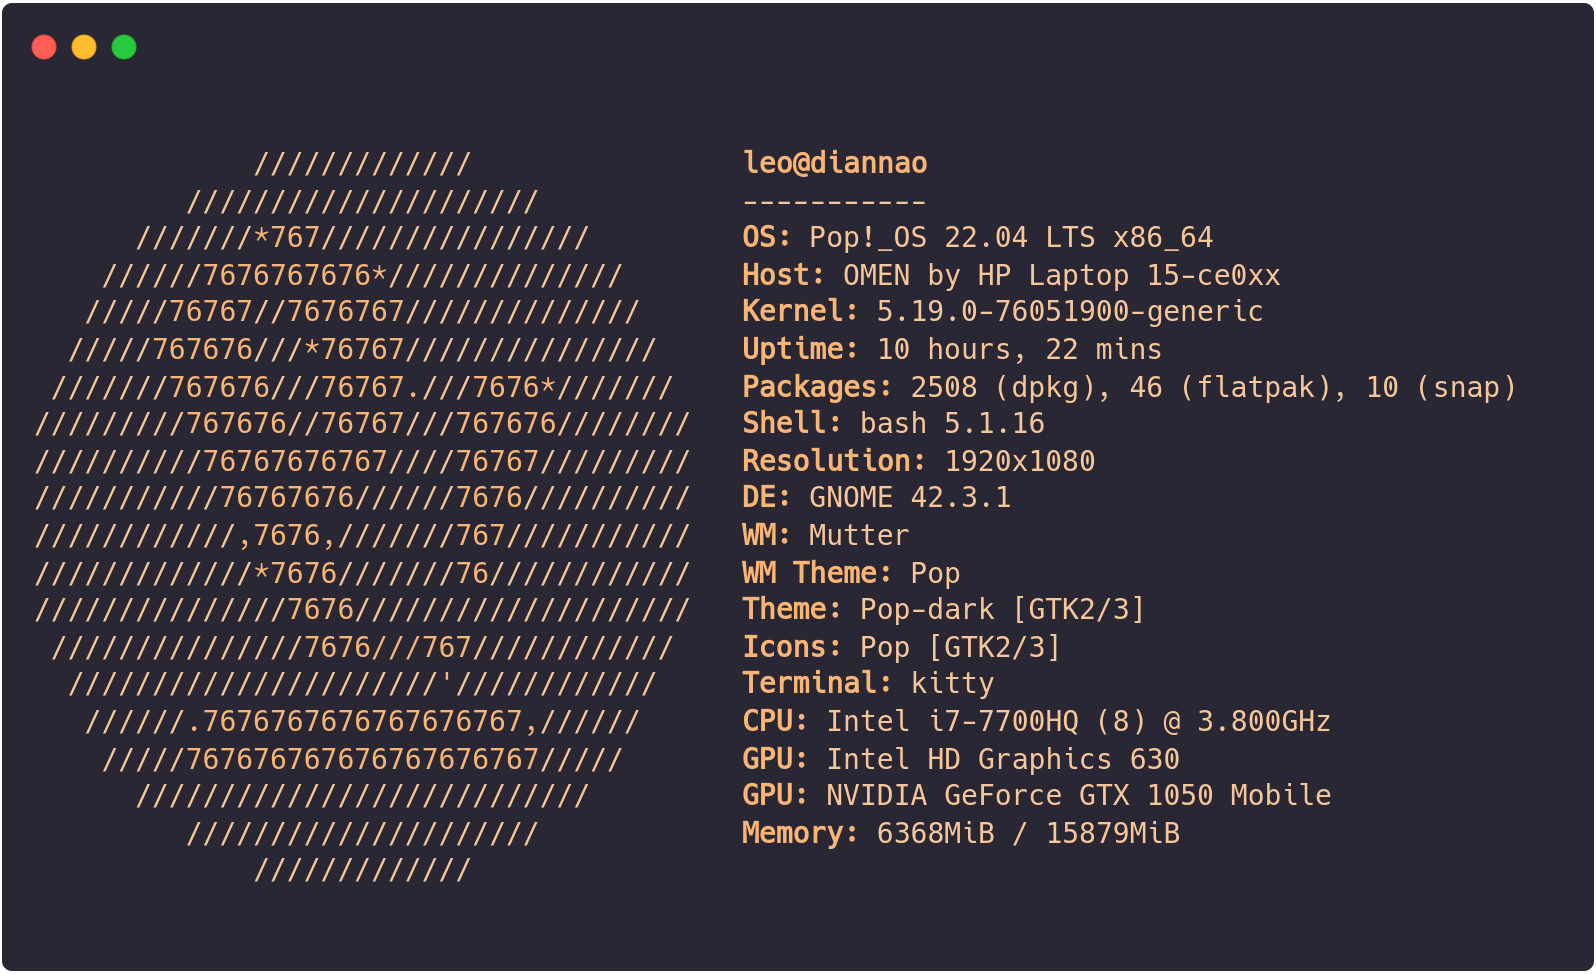
\includegraphics[scale=0.2]{../figures/diannao-specs}
    \caption{Características del ordenador {\diannao}.}
    \label{fig:diannao-specs}
\end{figure}
\begin{figure}[ht!]
    \centering
    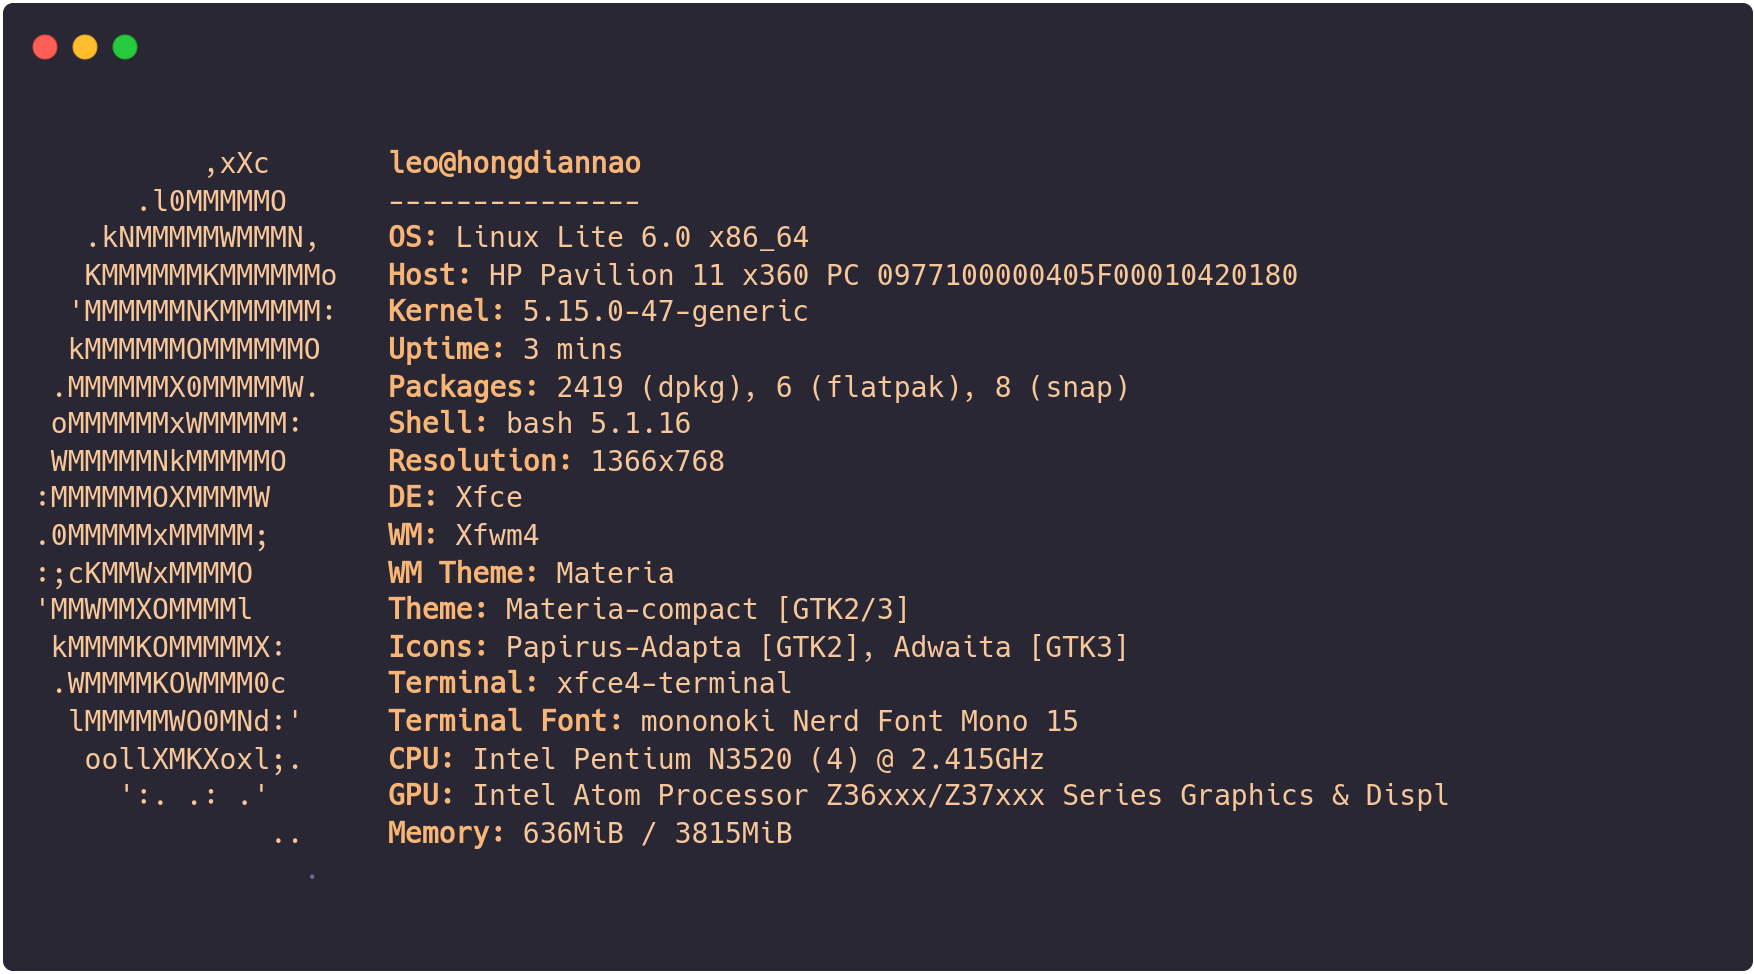
\includegraphics[scale=0.2]{../figures/hongdiannao-specs}
    \caption{Características del ordenador {\hongdiannao}.}
    \label{fig:hongdiannao-specs}
\end{figure}
Por último quisiera mencionar que \code{julia} no es un lenguage para hacer scripts, similar al modo de trabajo usando \code{python}. Por ello fue que se adjunto al inicio de esta tarea una demostración sobre como se usó el módulo en el apéndice para computar los tiempos requeridos en ambas computadoras. Se anexaron como demostración imagenes de fractales al final del trabajo, mientras más alto es el número máximo de iteraciones se obtiene una mejor coloración, y aumenta la definición de la imagen mientras más fino es el mallado. Las zonas que asemejan nubes de color son zonas en donde el mismo número de iteraciones se obtuvo.

\begin{figure}
    \centering
    \begin{subfigure}[t]{0.3\textwidth}
        \centering
        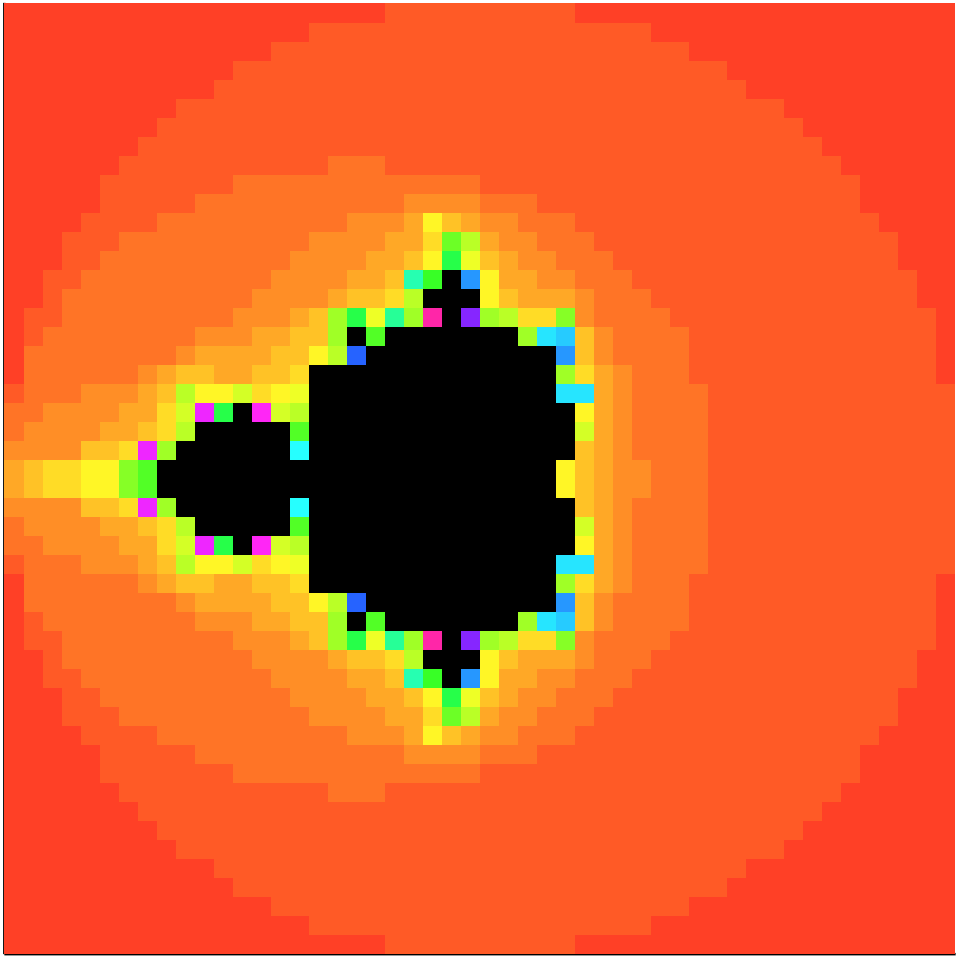
\includegraphics[scale=0.15]{../figures/fractal-n050-mx050}
        \caption{\code{nx} = \code{ny} = 50; \code{maxiter} = 50.}
    \end{subfigure}
    \begin{subfigure}[t]{0.3\textwidth}
        \centering
        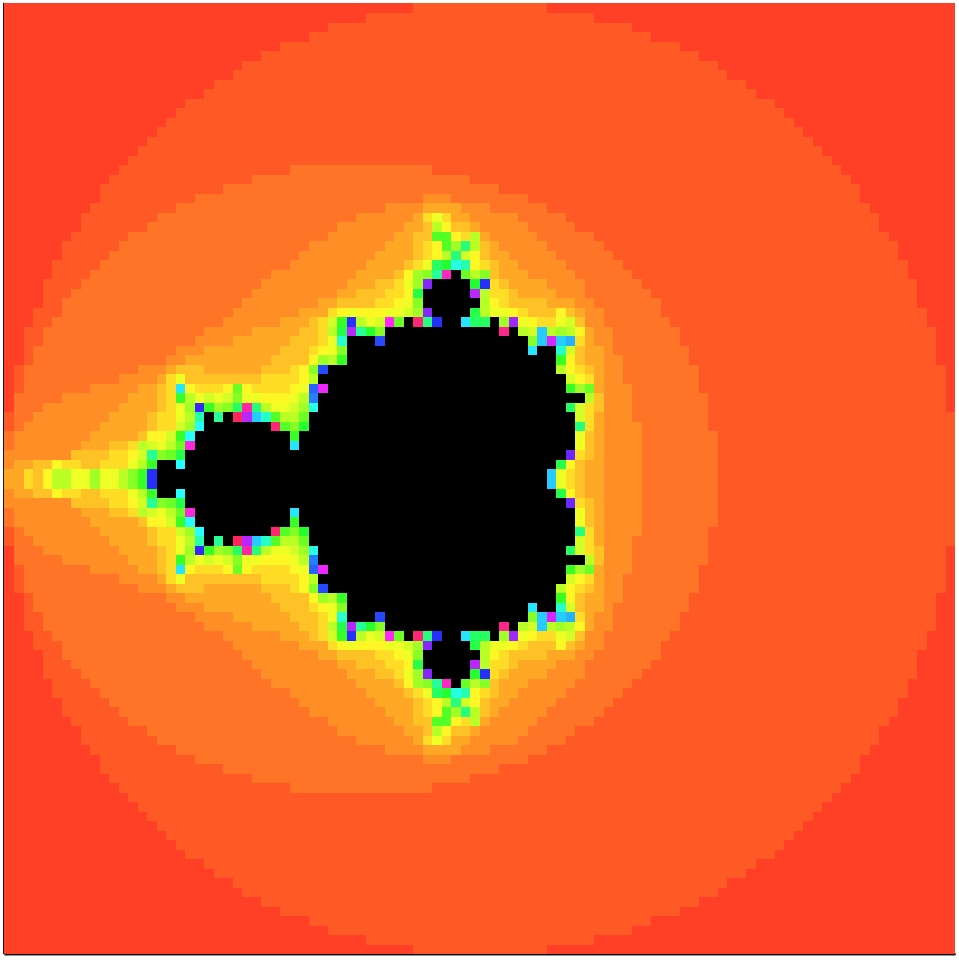
\includegraphics[scale=0.15]{../figures/fractal-n100-mx050}
        \caption{\code{nx} = \code{ny} = 100; \code{maxiter} = 50.}
    \end{subfigure}
    \begin{subfigure}[t]{0.3\textwidth}
        \centering
        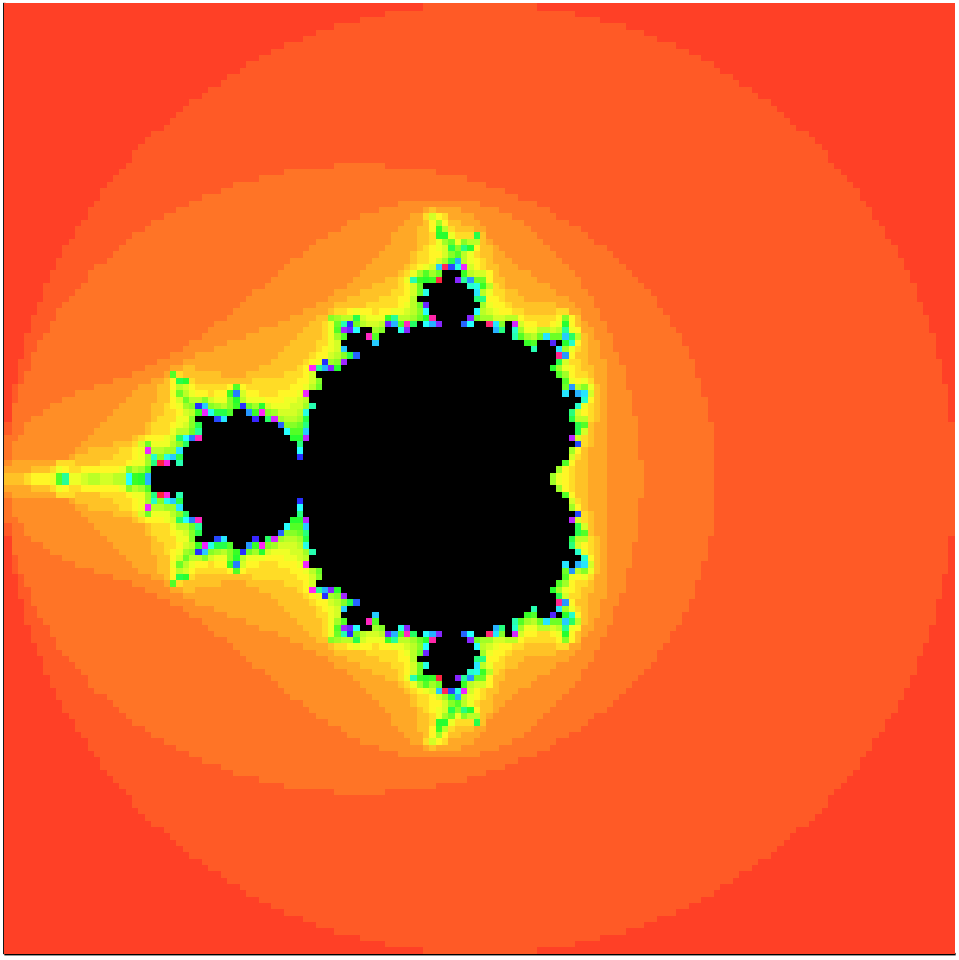
\includegraphics[scale=0.15]{../figures/fractal-n150-mx050}
        \caption{\code{nx} = \code{ny} = 150; \code{maxiter} = 50.}
    \end{subfigure}
    \begin{subfigure}[t]{0.3\textwidth}
        \centering
        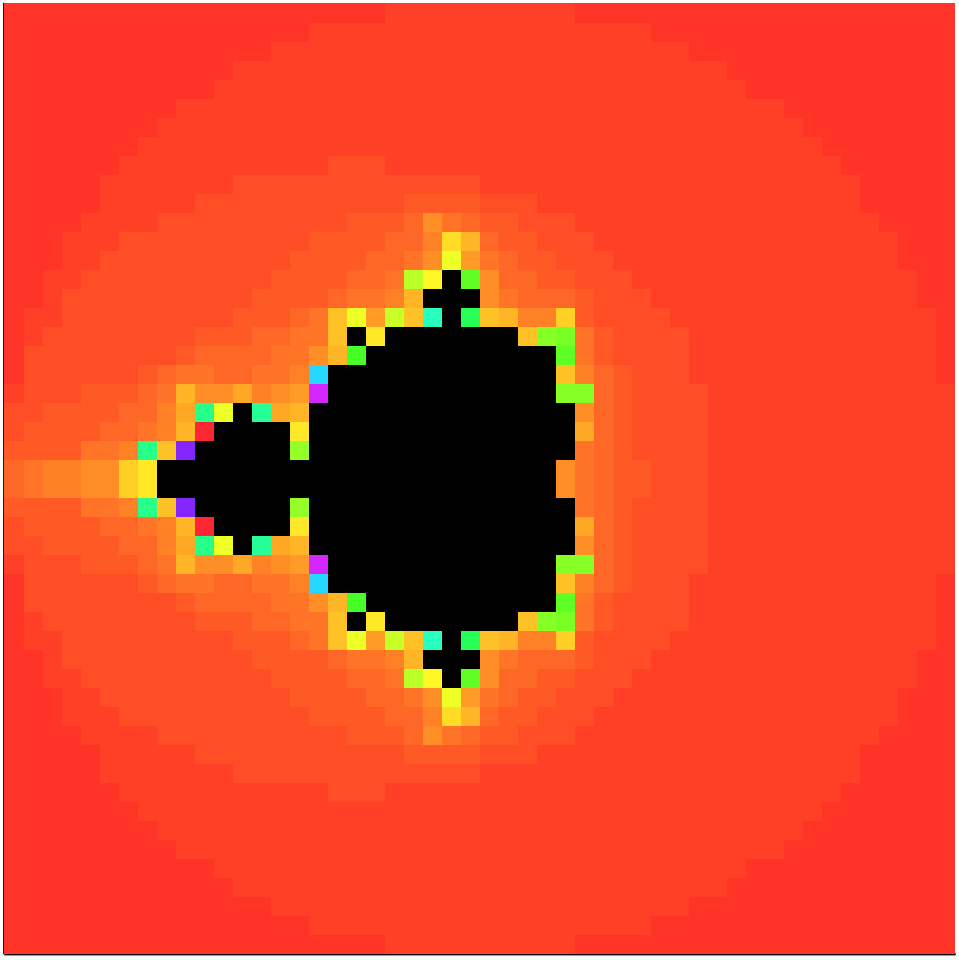
\includegraphics[scale=0.15]{../figures/fractal-n050-mx100}
        \caption{\code{nx} = \code{ny} = 50; \code{maxiter} = 100.}
    \end{subfigure}
    \begin{subfigure}[t]{0.3\textwidth}
        \centering
        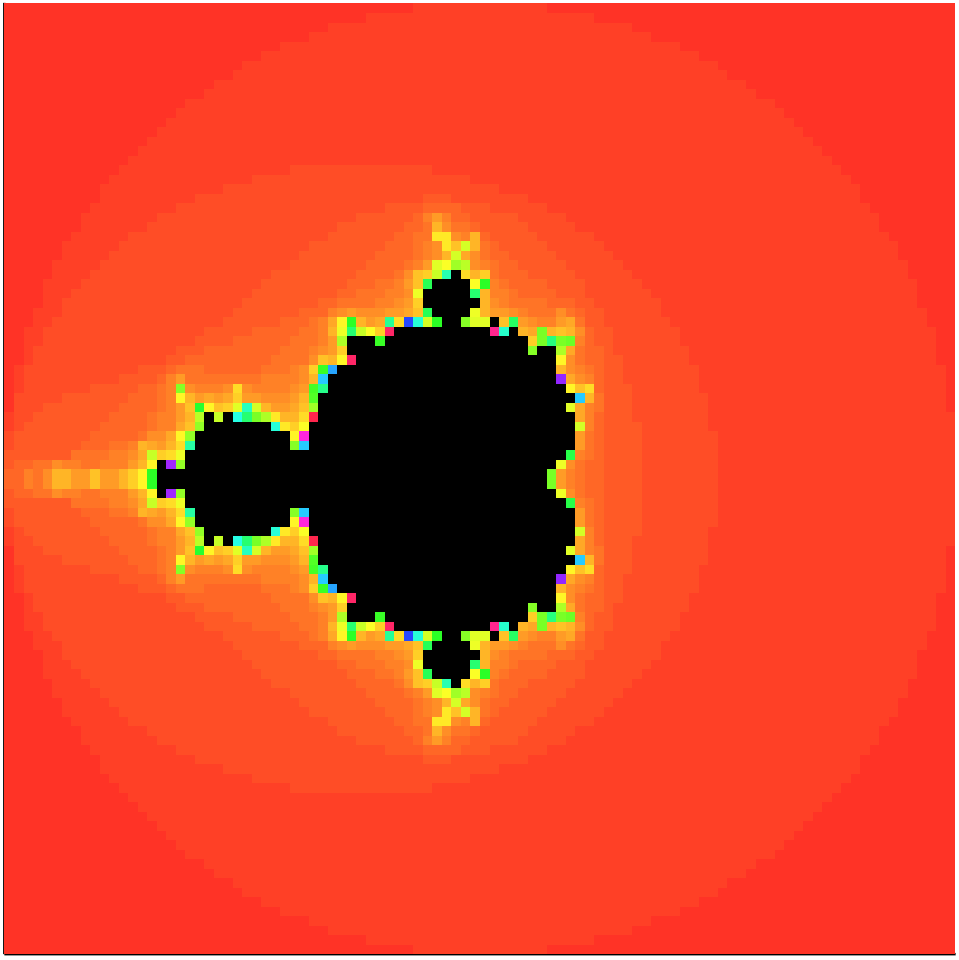
\includegraphics[scale=0.15]{../figures/fractal-n100-mx100}
        \caption{\code{nx} = \code{ny} = 100; \code{maxiter} = 100.}
    \end{subfigure}
    \begin{subfigure}[t]{0.3\textwidth}
        \centering
        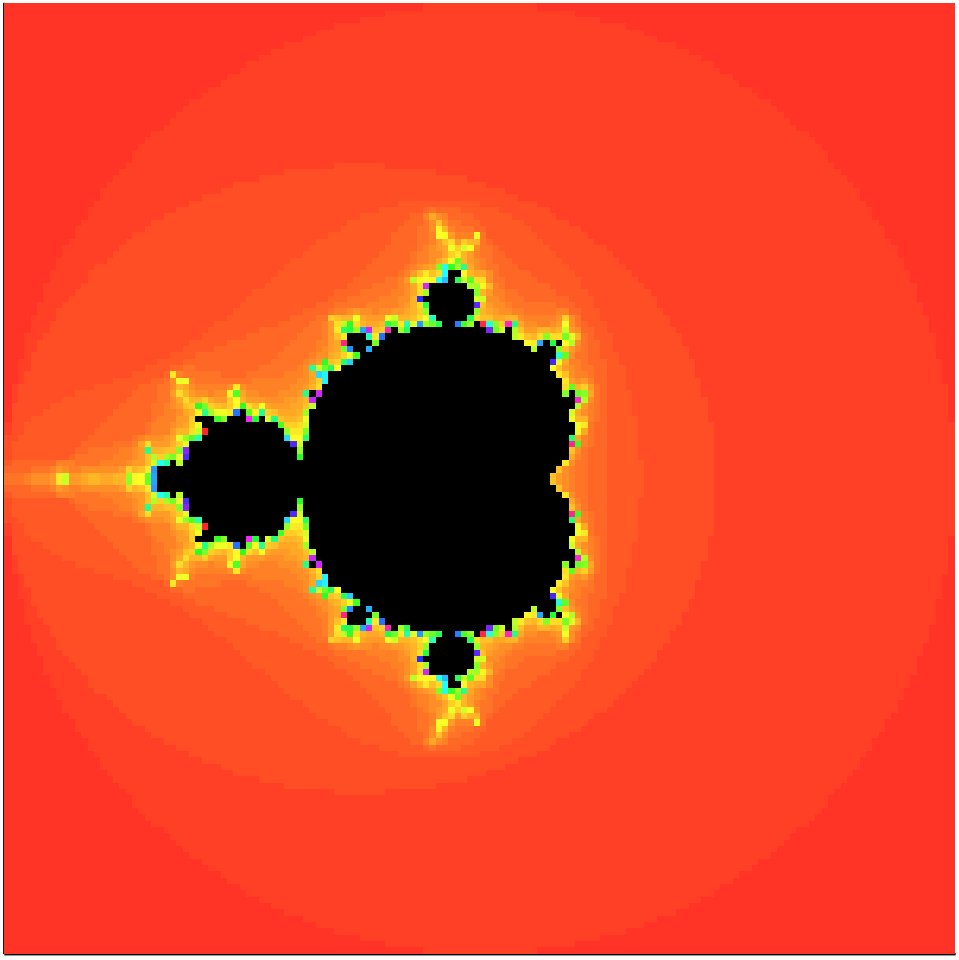
\includegraphics[scale=0.15]{../figures/fractal-n150-mx100}
        \caption{\code{nx} = \code{ny} = 150; \code{maxiter} = 100.}
    \end{subfigure}
    \begin{subfigure}[t]{0.3\textwidth}
        \centering
        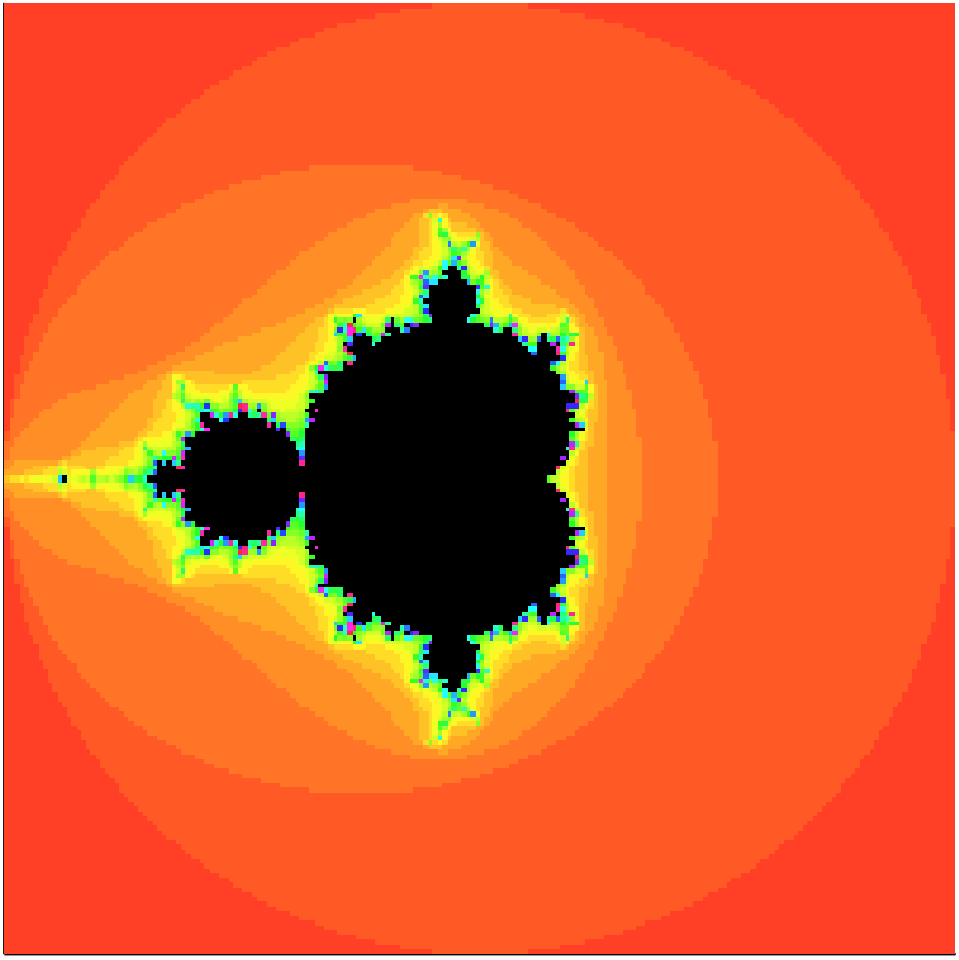
\includegraphics[scale=0.15]{../figures/fractal-n200-mx050}
        \caption{\code{nx} = \code{ny} = 200; \code{maxiter} = 50.}
    \end{subfigure}
    \begin{subfigure}[t]{0.3\textwidth}
        \centering
        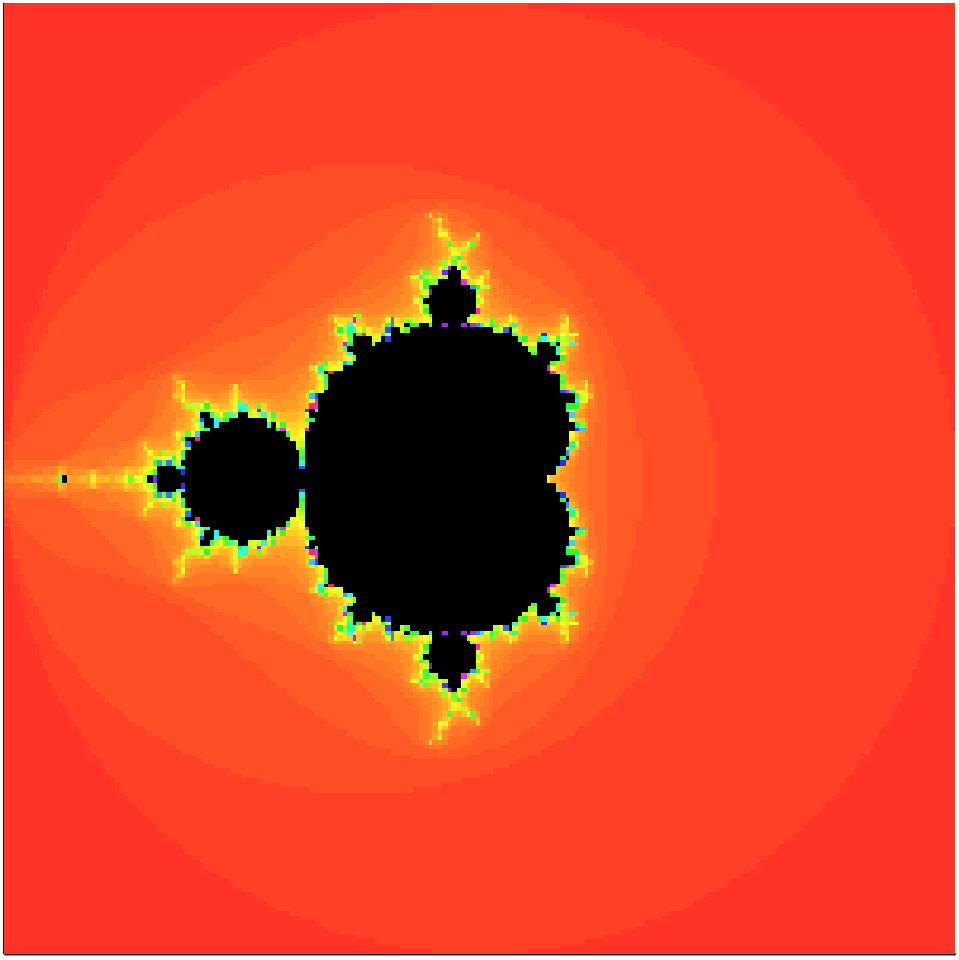
\includegraphics[scale=0.15]{../figures/fractal-n200-mx100}
        \caption{\code{nx} = \code{ny} = 200; \code{maxiter} = 100.}
    \end{subfigure}
    \caption{Ejemplos de fractales que se pueden obtener usando el módulo desarrollado. Se anexan sus condiciones iniciales.}
\end{figure}

\begin{figure}
    \centering
    \begin{subfigure}[b]{0.95\textwidth}
        \centering
        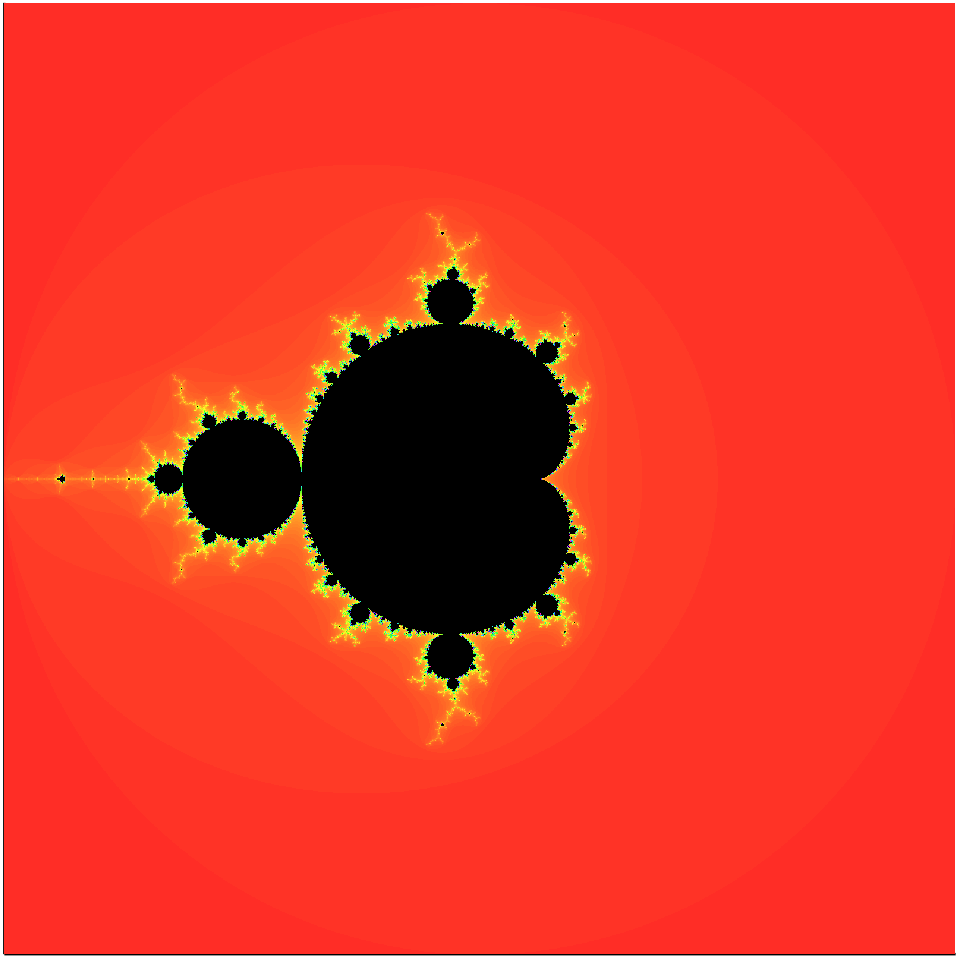
\includegraphics[scale=0.3]{../figures/fractal-n1600-mx200}
        \caption{\code{nx} = \code{ny} = 1600; \code{maxiter = 200}.}
    \end{subfigure}
    \begin{subfigure}[b]{0.95\textwidth}
        \centering
        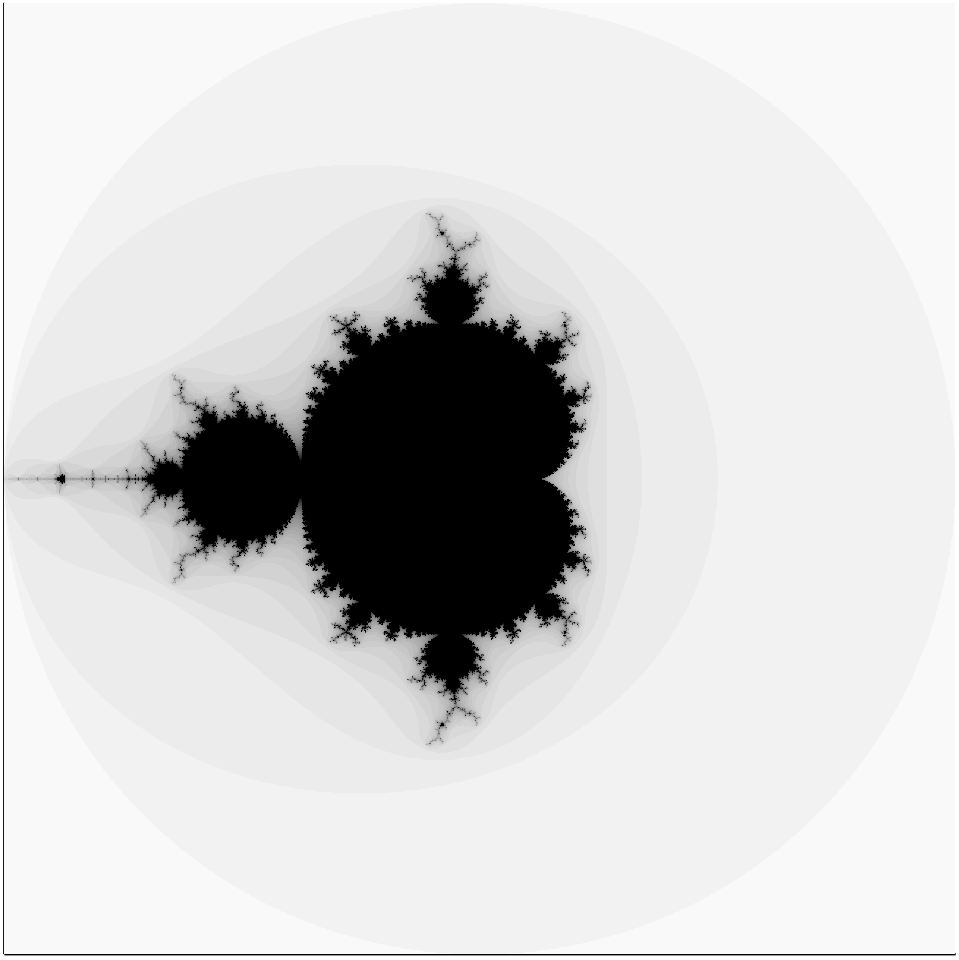
\includegraphics[scale=0.3]{../figures/fractal-n1600-mx040}
        \caption{\code{nx} = \code{ny} = 1600; \code{maxiter = 40}.}
    \end{subfigure}
    \caption{Fractales con mayor definición.}
\end{figure}

% \pagebreak
% -- BIBLIOGRAFIA
% \nocite{*} % to call all references even if they are not cited in the text
% \bibliography{references.bib}

\pagebreak
% -- Referencias
\section*{Referencias}
\begin{enumerate}[label={[\arabic*]}]
    \item Mandelbrot set. (20 Septiembre 2022). En Wikipedia. \\\url{https://en.wikipedia.org/wiki/Mandelbrot_set}
    \item Bezanson, J., Edelman, A., Karpinski, S., \& Shah, V. B. (2017). Julia: A fresh approach to numerical computing. SIAM Review, 59(1), 65–98. \url{https://doi.org/10.1137/141000671}
    \item Vladimir, R. F. H. (21 Septiembre 2022). Análisis de Algoritmos. Universidad Veracruzna.
\end{enumerate}

% -- CODIGO
\vspace{1cm}
\section*{Apéndice}
\inputminted[
    frame=none,
    % obeytabs=false,
    breaklines,
    tabsize=4,
    linenos=true,
    % numbersep=-10pt,
    baselinestretch=1,
    firstnumber=last,
    bgcolor=bg,
]{julia}{\codepath}


\end{document}